\documentclass[preprint,notitlepage]{revtex4-2}
\usepackage{amsmath, amssymb}
\usepackage{graphicx}
\usepackage{float}
\usepackage{booktabs}
\usepackage{xcolor}
\usepackage{tcolorbox}
\usepackage{hyperref}
\usepackage{enumitem}
\usepackage{physics}
\usepackage{caption}
\usepackage{bm}
\usepackage{tikz}
\usepackage{pgfplots}
\usepackage{lmodern}
\usepackage{amsmath,amssymb,amsfonts}
\usepackage{mathtools}
\usetikzlibrary{knots,intersections,decorations.pathreplacing}
\usetikzlibrary{3d, calc, arrows.meta, positioning}
\usepackage{pgfmath}
\usetikzlibrary{decorations.pathmorphing}
\pgfplotsset{compat=1.18} % or version you have
\usepackage{titlesec}
\usepackage{ulem}
\usepackage[utf8]{inputenc}
\usepackage[T1]{fontenc}
\renewcommand{\grqq}{``}


\begin{document}
\title{Revisiting the Æther:\\ From Einstein to the Vortex Fluid Paradigm}
\author{Omar Iskandarani\footnote{\scriptsize This paper is not intended as a neutral historical review, but as a conceptual bridge—framing the Vortex Æther Model (VAM) as a contemporary realization of Einstein’s late æther philosophy. \textbf{Keywords:} Æther, Einstein, Vortex fluid model, Time dilation, Topological gravity, Field theory, Helmholtz, Maxwell, Kelvin, unified field theory}}
\thanks{Independent Researcher, Groningen, The Netherlands\\
        info@omariskandarani.com \\
        ORCID: \href{https://orcid.org/0009-0006-1686-3961}{0009-0006-1686-3961} \\
        DOI: \href{https://doi.org/10.5281/zenodo.15669901}{10.5281/zenodo.15669901}}
\date{\today}
\maketitle

\begin{abstract}
This paper revisits the concept of the æther through Einstein’s post-1920 writings, culminating in a structured reinterpretation via the Vortex Æther Model (VAM). Contrary to the belief that Einstein abandoned the æther, we show that his later work restored it as a physically meaningful medium—devoid of mechanical motion but endowed with field-like properties essential for gravitation and inertia. We trace this shift from the 1905 rejection of the luminiferous æther to the 1924 Einstein–Cartan correspondence, emphasizing its continuity with modern field-theoretic frameworks.

VAM builds on this foundation by modeling the æther as an incompressible, inviscid superfluid. Gravitation and inertia emerge from the quantized circulation of knotted vortex filaments, with vorticity replacing curvature as the physical substrate of gravitational effects. Conserved angular momentum gives rise to time dilation, inertial response, and mass-energy equivalence. We define an effective mass profile \( M_{\text{eff}}(r) = \int_0^r 4\pi r'^2 \rho_\text{\ae}^{(\text{energy})}(r') \, dr' \), derived from localized vortex energy, and introduce a swirl potential \( \Omega(r) = \frac{C_e}{r_c} e^{-r/r_c} \), which governs fluid-mediated gravitation via Bernoulli-like pressure gradients.

Time dilation arises from tangential vortex flow as \( \frac{d\tau}{dt} = \sqrt{1 - \frac{v_\theta^2}{c^2}} \), with \( v_\theta(r) = \frac{\Gamma}{2\pi r} \), where \( \Gamma \) is the circulation quantum and \( v_\theta \) the local swirl velocity. This expression recovers relativistic time effects from fluid kinematics, without invoking curvature.

This sets a conceptual and mathematical foundation for VAM, in which classical and quantum behavior emerge from topological fluid dynamics. The model distinguishes three temporal modes within the æther: \( \mathcal{N} \) (Æther-Time), \( \tau \) (Proper Time), and \( S(t) = \int \Omega(r)\, dt \) (Swirl Clock Phase), offering a layered ontology of temporality. For empirical benchmarking against general relativity, see the companion analysis in~\cite{VAM-3}.
\end{abstract}

\section{Introduction}
\section{Introduction}\label{sec:inleiding}

Despite the empirical success of the Standard Model (SM) of particle physics and General Relativity (GR), fundamental questions remain unresolved: What is the physical origin of mass? Why do gauge interactions exhibit their particular symmetries? What gives rise to natural constants such as $\hbar$, $e$, or $\alpha$ beyond dimensional convenience?

Mainstream physics relies heavily on abstract mathematical formalisms—such as symmetry groups, Lagrangian terms, and quantum operators—that, while predictive, often obscure the underlying physical ontology. This paper proposes an alternative: the \emph{Vortex Æther Model} (VAM), a mechanistic, fluid-dynamic framework in which spacetime and all physical phenomena emerge from structured motion in a compressible, superfluid-like æther.

In VAM, elementary particles are not point-like fields but stable, knotted vortex structures embedded in the æther. Observable properties such as mass, charge, spin, and flavor are reinterpreted as topological and dynamical characteristics—circulation strength, core radius, swirl helicity—of these vortex knots. Gauge and Higgs interactions are expressed as manifestations of fluid tension, reconnection, and swirl transfer.

Crucially, this is not merely a reformulation of mathematical symbols. The goal of VAM is to provide an \emph{ontological replacement} for conventional quantum field theory: a physically intuitive, testable substrate from which all constants and couplings emerge. Within this framework, the Standard Model is reconstructed from five physically meaningful ætheric quantities: swirl velocity $C_e$, core radius $r_c$, æther density $\rho_\text{\ae}$\footnote{The VAM framework distinguishes between three æther densities depending on context: fluid, energy, and mass-equivalent. See Table~\ref{tab:ae_densities_foot} for a breakdown of these definitions. A mismatch in interpretation leads to inconsistencies in field derivations.}, maximum force $F^{\text{max}}_{\text{\ae}}$, and circulation $\Gamma$.

This paper presents a full reformulation of the Standard Model Lagrangian using these VAM-derived units and fields. Each term acquires a mechanical and geometric interpretation, leading to a unified description where quantum phenomena, gauge structures, and mass generation are consequences of vortex dynamics in an inviscid æther. A full field-theoretic derivation of the model dynamics is presented in Appendix~\ref{sec:EL-derivation}.

Historically, this effort revives foundational ideas from Kelvin's vortex-atom hypothesis and Maxwell's æther mechanics, updating them within a modern context informed by quantum fluids, superfluid analogs of gravity, and topological field theory. See, for example, Volovik's emergent gravity framework in helium II~\cite{Volovik2003UniverseInHelium}, Barceló et al.'s review of analog spacetime geometries~\cite{Barcelo2005AnalogueGravityReview}, and Kleckner and Irvine's experimental realization of knotted vortices~\cite{Kleckner2013KnottedVortices}. While this paper is designed to be standalone, these works contextualize the broader landscape of fluid-based physical models.

By grounding the abstract structures of modern physics in vortex geometry, VAM aims to bridge the gap between formal theory and intuitive physical mechanisms—offering not only reinterpretation, but a re-foundation of particle physics itself.

This work builds on a series of earlier papers developing the Vortex Æther Model (VAM). In \cite{iskandarani2025timedilation}, proper time was defined through internal angular motion of vortex cores, introducing the concept of \("\)swirl clocks\("\) as the microscopic origin of time dilation. This was extended in \cite{iskandarani2025swirlgravity}, which proposed that gradients in swirl clocks — arising from non-uniform vorticity — mimic gravitational curvature, including analogs to event horizons. The present work synthesizes these concepts into a variational field-theoretic framework, reformulating the Standard Model Lagrangian in terms of helicity, core structure, and topological æther dynamics.

\subsection*{Postulates of the Vortex Æther Model}
\begin{table}[h!]
    \centering
    \begin{tabular}{rl}
        \hline
        \textbf{1. Continuous Space} & Space is Euclidean, incompressible and inviscid. \\
        \textbf{2. Knotted Particles} & Matter consists of topologically stable vortex nodes. \\
        \textbf{3. Vorticity} & The vortex circulation is conserved and quantized. \\
        \textbf{4. Absolute Time} & Time flows uniformly throughout the æther. \\
        \textbf{5. Local Time} & Time is locally slower due to pressure and vorticity gradients. \\
        \textbf{6. Gravity} & Emerges from vorticity-induced pressure gradients. \\
        \hline
        \bottomrule
    \end{tabular}
    \caption{Postulates of the Vortex Æther Model (VAM).}
    \label{tab:postulates}
\end{table}

The postulates replace spacetime curvature with structured rotational flows and thus form the foundation for emergent mass, time, inertia, and gravity.

\section*{Terminology and Classical Correspondence}

We introduce several novel constructs to describe the vortex-based field framework. For clarity, Table~\ref{tab:vam_definitions} provides precise definitions and links to standard physics concepts.

\begin{table}[H]
    \centering
    \scriptsize
    \renewcommand{\arraystretch}{1.3}
    \begin{tabular}{|l|l|l|}
        \hline
        \textbf{Term} & \textbf{Definition in VAM} & \textbf{Analogy in Established Theory} \\
        \hline
        \makecell[l]{Swirl Clock} &
        \makecell[l]{Proper time defined by internal angular frequency \\ $\omega_0$ of a vortex core} &
        \makecell[l]{Atomic clock (GR); spin-precession \\ in gyroscopes} \\
        \hline
        \makecell[l]{Swirl Lagrangian} &
        \makecell[l]{Field Lagrangian including helicity term \\ $\lambda (\mathbf{v} \cdot \boldsymbol{\omega})$} &
        \makecell[l]{Chern–Simons terms; \\ topological terms in QFT} \\
        \hline
        \makecell[l]{Helicity Time} &
        \makecell[l]{Clock rate modulated by helicity density: \\ $d\tau \propto \mathbf{v} \cdot \boldsymbol{\omega}$} &
        \makecell[l]{Phase evolution in rotating frames; \\ action-angle methods} \\
        \hline
        \makecell[l]{Core Radius $r_c$} &
        \makecell[l]{Characteristic radius of maximal vorticity \\ and core energy density} &
        \makecell[l]{Healing length in BECs; \\ flux tube radius in QCD} \\
        \hline
        \makecell[l]{Swirl Speed $C_e$} &
        \makecell[l]{Tangential speed of æther flow \\ at core radius} &
        \makecell[l]{Sound speed in superfluids; \\ Lorentz frame velocity} \\
        \hline
        \makecell[l]{Swirl Horizon} &
        \makecell[l]{Boundary beyond which $\omega_{\text{obs}} \to 0$ \\ and clocks stall} &
        \makecell[l]{GR event horizon; \\ ergosphere boundary (Kerr geometry)} \\
        \hline
    \end{tabular}
    \caption{Key theoretical constructs in the Vortex Æther Model (VAM), mapped to classical and quantum analogs for interpretability.}
    \label{tab:vam_definitions}
\end{table}


These constructs provide an intuitive bridge between fluid mechanics, quantum field theory, and emergent spacetime phenomena, facilitating reinterpretation of the Standard Model Lagrangian in a vortex-based æther framework.

\section{Reevaluating Einstein’s Supposed Rejection of the Æther}
\input{02_Rejection_Æther}

\section{Multimodal Time: The Ætheric Temporal Ontology}
The Vortex Æther Model (VAM) advances a multimodal conception of time, rooted in the internal and relational dynamics of an incompressible, inviscid æther. Unlike the unidimensional time parameter in standard field theory or the proper time of General Relativity, VAM’s temporal taxonomy encapsulates distinct physical, topological, and informational modes, each with a clear analytical and experimental role. This layered approach not only extends Einstein’s “geometric æther” but also provides a framework for modeling causality, memory, and quantum-classical transitions in a unified manner~\cite{VAM-8, VAM-13, VAM-15}.

\begin{figure}[htb]
    \centering
    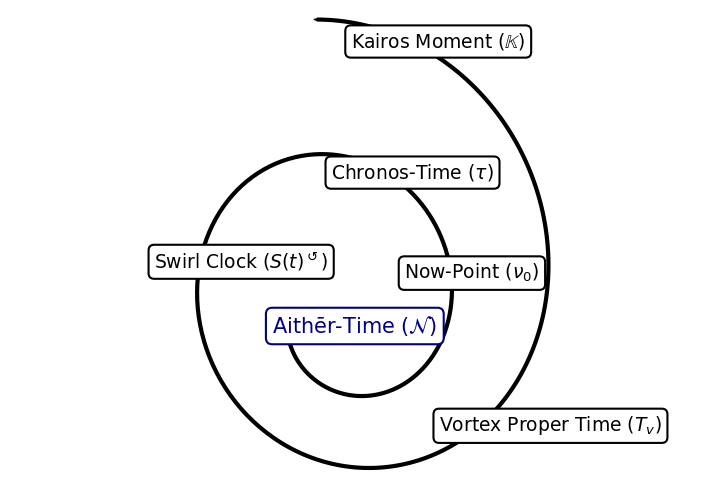
\includegraphics[width=0.7\textwidth]{TemporalOntology}
    \caption{
        \textbf{Vortex Phase Spiral of Ætheric Time.} This figure illustrates the sequential emergence of layered temporal modes in the VAM framework, with each governing a distinct aspect of physical law. The progression radiates outward from Aithēr-Time ($\boldsymbol{\mathcal{N}}$), through Now-Point ($\boldsymbol{\nu_0}$), Chronos-Time ($\boldsymbol{\tau}$), Swirl Clock ($\boldsymbol{S}^{\boldsymbol{\circlearrowleft}}_\text{(t)}$), and Vortex Proper Time ($\boldsymbol{T_v}$), to the outermost Kairos Moment ($\mathbb{\boldsymbol{K}}$). These layers form a unified temporal architecture foundational to vortex dynamics~\cite{VAM-8, VAM-13}.
    }

    \label{fig:temporal_ontology}
\end{figure}

The multimodal temporal ontology of VAM is not purely an abstract taxonomy; it possesses a geometric and topological structure, naturally visualized as a multidimensional “spiral” or “fan” in phase space (see Fig.~\ref{fig:temporal_ontology}). This structure parallels phase-space geometries explored in superfluid analog gravity and topological vacua~\cite{volovik2003universe}. Each temporal mode—Aithēr-Time, Now-Point, Chronos-Time, Swirl Clock, Vortex Proper Time, and Kairos Moment—plays an independent yet interconnected role, governing different layers of physical law~\cite{VAM-8, VAM-13}.

\begin{tcolorbox}[
  colback=gray!10,
  colframe=black,
  width=1.0\textwidth,
  sharp corners=southwest,
  boxrule=0.5pt,
  before skip=10pt,
  after skip=10pt,
  title=\textbf{Table: Ætheric Time Modes in the Vortex Æther Model},
  fonttitle=\bfseries,
]
\renewcommand{\arraystretch}{1.25}
\small
\begin{tabular}{r l l}
  $\boldsymbol{\mathcal{N}}$     & \textbf{Aithēr-Time}         & Absolute causal ordering parameter~\cite{VAM-8, VAM-13} \\
  $\boldsymbol{\nu_0}$           & \textbf{Now-Point}           & Localized intersection with universal present~\cite{VAM-8, VAM-13} \\
  $\boldsymbol{\tau}$            & \textbf{Chronos-Time}        & Measurable time in the æther (subject to dilation)~\cite{VAM-1, VAM-8} \\
  $\boldsymbol{S}^{\boldsymbol{\circlearrowleft}}_\text{(t)}$ & \textbf{Swirl Clock}         & Internal phase memory of a vortex~\cite{VAM-2, VAM-13, VAM-15} \\
  $\boldsymbol{T_v}$             & \textbf{Vortex Proper Time}  & Circulation-based geodesic duration~\cite{VAM-2, VAM-13} \\
  $\mathbb{\boldsymbol{K}}$      & \textbf{Kairos Moment}       & Discrete topological bifurcation event~\cite{VAM-13, VAM-15} \\
\end{tabular}
\end{tcolorbox}

\noindent The interpretation of each mode is as follows:
\begin{itemize}
    \item \textbf{Aithēr-Time ($\boldsymbol{\mathcal{N}}$):} The unobservable but indispensable global time parameter that orders all events causally within the ætheric manifold, serving as the absolute temporal background for physical processes~\cite{VAM-8, VAM-13}.

    \item \textbf{Now-Point ($\boldsymbol{\nu_0}$):} The localized realization of the present, defined by the intersection of the global time field $\boldsymbol{\mathcal{N}}$ with a point in the æther manifold. It establishes the surface of simultaneity and facilitates causal foliation~\cite{VAM-8, VAM-13}.

    \item \textbf{Chronos-Time ($\boldsymbol{\tau}$):} The physically measurable flow of time, experienced within the æther and modulated by local vorticity through swirl-induced time dilation~\cite{VAM-1, VAM-8}:
    \[
        \frac{d\boldsymbol{\tau}}{dt} = \sqrt{1 - \boldsymbol{v_\phi}^2(r)/c^2}
    \]
    where $\boldsymbol{v_\phi}(r)$ is the local tangential velocity of the vortex field.

    \item \textbf{Swirl Clock ($\boldsymbol{S}^{\boldsymbol{\circlearrowleft}}_\text{(t)}$):} The internal phase variable of a vortex structure, tracking angular displacement and serving as a memory function for topological identity and history, drawing from foundational work on helicity conservation and knot topology in vortex dynamics~\cite{knot_theroy_in_fluid}. It is formally given by~\cite{VAM-2, VAM-13}:
    \[
        \boldsymbol{S}^{\boldsymbol{\circlearrowleft}}_\text{(t)} = \int_{0}^{t} \boldsymbol{\Omega}(r(t'))\, dt'
    \]
    with $\boldsymbol{\Omega}(r)$ the local angular velocity.

    \item \textbf{Vortex Proper Time ($\boldsymbol{T_v}$):} The intrinsic circulation-based duration associated with a closed path around a vortex core, defined as~\cite{VAM-2, VAM-13}
    \[
        \boldsymbol{T_v} = \oint \frac{dl}{\boldsymbol{v_\phi}(r)}
    \]
    representing the intrinsic “clock” of a knotted structure.

    \item \textbf{Kairos Moment ($\mathbb{\boldsymbol{K}}$):}
    The discrete event marking a topological transition such as vortex reconnection or bifurcation, producing an irreversible change in vortex identity and introducing discontinuities or non-analyticities in the evolution of $\boldsymbol{T_v}$ or $\boldsymbol{S}^{\boldsymbol{\circlearrowleft}}_\text{(t)}$~\cite{VAM-13, VAM-15}.
\end{itemize}

In the VAM framework, the “Kairos Moment” ($\mathbb{\boldsymbol{K}}$) represents a discrete, topologically induced transition in the evolution of vortex matter—such as a vortex reconnection, bifurcation, or the passage of a gravitational wave. These events break the smooth evolution of then Swirl Clock phase and manifest as quantized phase slips or time jumps. As shown in Fig.~\ref{fig:kairos_moment}, a Kairos event appears as an abrupt change in the Swirl Clock trajectory during a localized temporal window~\cite{buhler2005wave}. Such phenomena are experimentally accessible in analog systems and may be detectable in astrophysical settings as phase anomalies or decoherence events in quantum or classical fields~\cite{VAM-13, VAM-15}. Such temporally localized events have been explored in analogue spacetime geometries where topological phase changes mimic gravitational discontinuities~\cite{barcelo2005}.


\begin{figure}[htb]
    \centering
    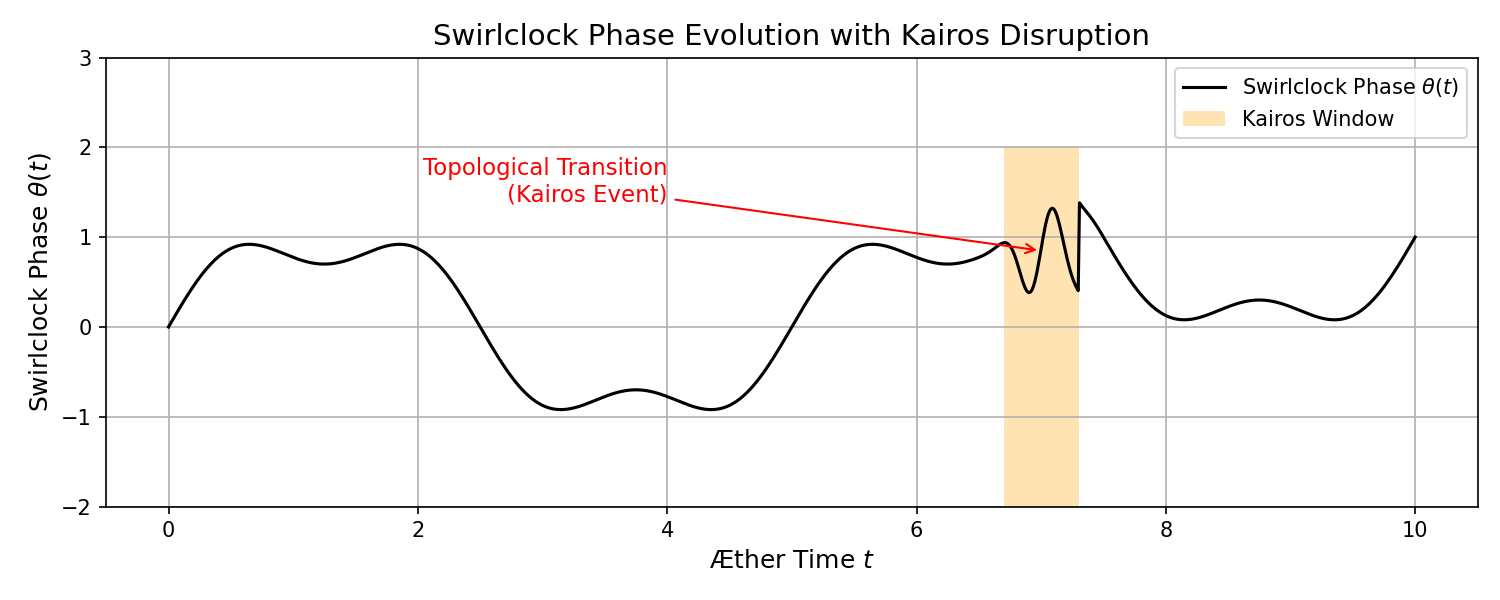
\includegraphics[width=0.7\textwidth]{TemporalOntologyKairosMoment}
    \caption{
        \textbf{Swirl Clock Phase Evolution with Kairos Disruption.}
        This figure illustrates the evolution of the Swirl Clock phase, \(\theta(t)\), as a function of Æther Time (\(t
        \)), within the VAM temporal framework. A discrete topological transition—such as vortex reconnection or a passing gravitational wave—introduces a discontinuity in the otherwise smooth phase trajectory.
        The highlighted region, labeled the “Kairos Window,” marks the critical temporal interval where this event occurs. Within this window, the
    vortex structure undergoes an irreversible bifurcation, producing a quantized phase slip or decoherence effect. Such phenomena are defined in VAM as “Kairos Moments” (\(\mathbb{{K}}\)).
        These moments represent a topologically-induced departure from deterministic phase continuity, signaling a transition to a new dynamical regime. Observable manifestations include time “jumps,” phase anomalies, or memory resets within vortex-based systems. Analog experiments in superfluid systems may provide empirical access to these signatures~\cite{VAM-13, VAM-15}.
    }
    \label{fig:kairos_moment}
\end{figure}

This multimodal temporal ontology enables VAM to bridge metaphysical continuity with physically testable vortex dynamics. It underpins several core applications in the extended VAM literature, including models of causality, gravitational time dilation, vortex identity, and swirl-induced phase decoherence~\cite{VAM-1, VAM-2, VAM-8, VAM-13, VAM-15}. For detailed derivations, see~\cite{VAM-2, VAM-8, VAM-13, VAM-15}.

\section{Connection to the Vortex Æther Model (VAM)}
The Vortex Æther Model (VAM), developed by O. Iskandarani since 2012, models the æther as an incompressible, non-viscous superfluid~\cite{VAM-8, VAM-13}. Within this framework, vorticity is elevated to a fundamental quantity that governs time dilation, inertial mass, and gravitational interaction~\cite{VAM-2, VAM-10, VAM-13}. Echoing Einstein’s 1920 redefinition of the æther as a physical substratum, VAM treats the æther as a structured, causal medium from which all dynamical behavior emerges~\cite{VAM-8}.

Key structural elements of VAM include:
\begin{itemize}
    \item \textbf{Topological structures} (e.g., knots, trefoils) representing stable particle identities and quantum numbers~\cite{VAM-8, VAM-11, VAM-14},
    \item \textbf{Time dilation} arising from swirl intensity near vortex cores~\cite{VAM-2, VAM-13},
    \item \textbf{A revised system of natural constants}, including $C_e$ (vortex boundary velocity) and $F^{\max}_{\text{\ae}}$ (maximum ætheric stress), defined and operationalized in the topological Lagrangian~\cite{VAM-14}.
\end{itemize}

Figure~\ref{fig:taxonomy} illustrates the classification flow based on topology, chirality, and tension within the swirl field framework.


\begin{figure}[!ht]
    \centering
    \footnotesize
    \scalebox{0.75}{
        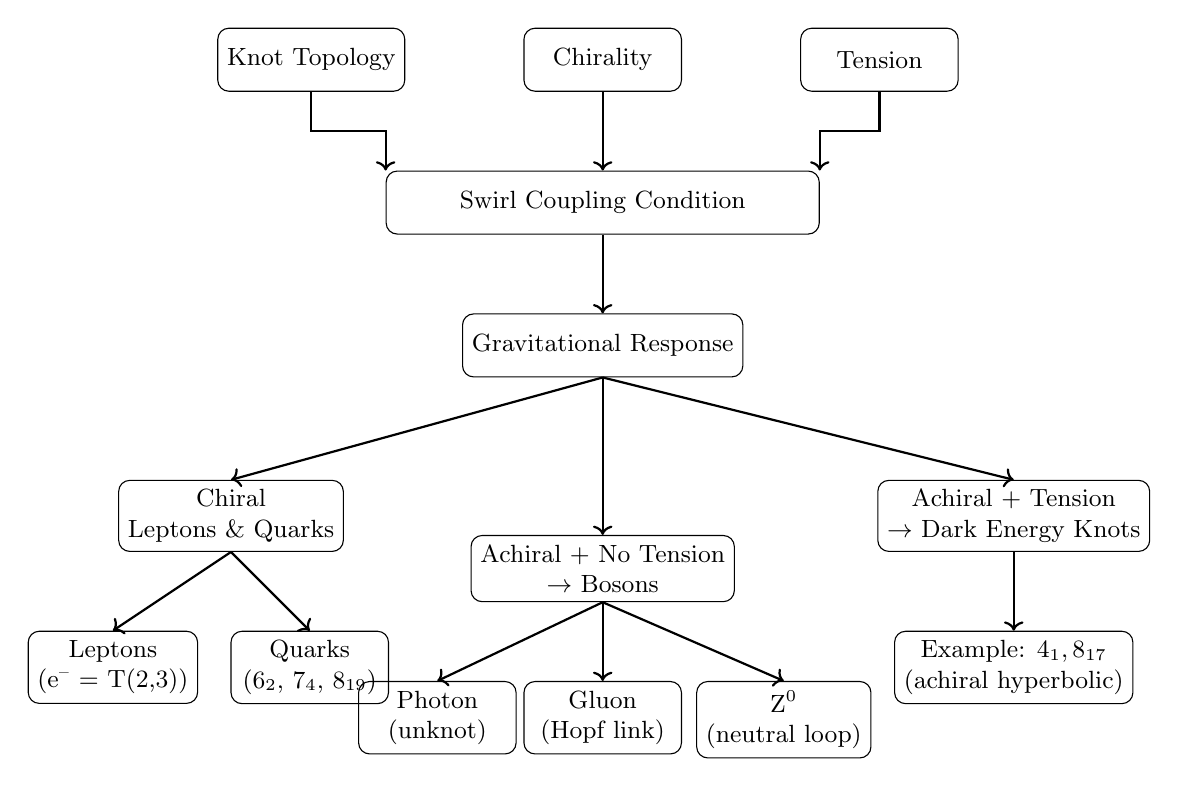
\begin{tikzpicture}[
          box/.style = {draw, rounded corners, minimum width=2.0cm, minimum height=0.8cm, font=\small, align=center},
          arrow/.style = {->, thick},   node distance=1.0cm and 1.5cm
        ]
            % Inputs
            \node[box] (topology) {Knot Topology};
            \node[box, right=of topology] (chirality) {Chirality};
            \node[box, right=of chirality] (tension) {Tension};

            % Swirl coupling
            \node[box, below=of chirality, minimum width=5.5cm] (coupling) {Swirl Coupling Condition};

            % Gravitational response
            \node[box, below=of coupling] (grav) {Gravitational Response};

            % Gravitational classes
            \node[box, below left=1.3cm and 1.5cm of grav] (matter) {Chiral\\Leptons \& Quarks};
            \node[box, below=2cm of grav] (boson) {Achiral + No Tension\\\(\rightarrow\) Bosons};
            \node[box, below right=1.3cm and 1.7cm of grav] (dark) {Achiral + Tension\\\(\rightarrow\) Dark Energy Knots};

            % Subclasses
            \node[box, below=of matter, xshift=-1.5cm] (leptons) {Leptons\\(e\textsuperscript{--} = T(2,3))};
            \node[box, below=of matter, xshift=+1.0cm] (quarks) {Quarks\\(6\textsubscript{2}, 7\textsubscript{4}, 8\textsubscript{19})};

            \node[box, below=of boson, xshift=-2.1cm] (photon) {Photon\\(unknot)};
            \node[box, below=of boson] (gluon) {Gluon\\(Hopf link)};
            \node[box, below=of boson, xshift=+2.3cm] (zboson) {Z\textsuperscript{0}\\(neutral loop)};

            \node[box, below=of dark] (darkex) {Example: \(4_{1}, 8_{17}\)\\ (achiral hyperbolic)};

            % Arrows to coupling
            \draw[arrow] (topology.south) -- ++(0,-0.5) -| (coupling.north west);
            \draw[arrow] (chirality.south) -- (coupling.north);
            \draw[arrow] (tension.south) -- ++(0,-0.5) -| (coupling.north east);

            % Arrows down flow
            \draw[arrow] (coupling.south) -- (grav.north);
            \draw[arrow] (grav.south) -- (matter.north);
            \draw[arrow] (grav.south) -- (boson.north);
            \draw[arrow] (grav.south) -- (dark.north);

            % Particle branches
            \draw[arrow] (matter.south) -- (leptons.north);
            \draw[arrow] (matter.south) -- (quarks.north);

            \draw[arrow] (boson.south) -- (photon.north);
            \draw[arrow] (boson.south) -- (gluon.north);
            \draw[arrow] (boson.south) -- (zboson.north);

            \draw[arrow] (dark.south) -- (darkex.north);
        \end{tikzpicture}
    }
    \caption{
        \textbf{Knot Classification by Swirl Coupling.}
        This flow diagram illustrates how fundamental particle types in the VAM framework emerge from topological features of vortex knots. (See classification list below.)
    }
    \label{fig:taxonomy}

\end{figure}

\vspace{0.1em}
\textbf{Classification summary:}
Knot topology, chirality, and curvature tension collectively determine a knot’s gravitational and inertial response, enabling classification into Standard Model families:
\begin{itemize}
    \item \textbf{Chiral knots} align with swirl fields and give rise to matter: \textbf{Leptons} (e.g., torus knots like \( T(2,3) \)), \textbf{Quarks} (e.g., hyperbolic knots like \( 5_2, 6_1, 8_{19} \)).
    \item \textbf{Achiral, tensionless} structures (unknots, Hopf links): \textbf{bosons}.
    \item \textbf{Achiral knots with intrinsic tension}: expelled, possible \textbf{dark energy} candidates (\( 4_1, 8_{17} \)).
\end{itemize}
\vspace{0.3em}

The classification is governed by the Swirl Coupling Condition, connecting geometric knot invariants to physical properties such as mass, spin, and interaction profile.

Knot theory has long informed fluid dynamics and topological invariants in vorticity~\cite{knot_theroy_in_fluid}, providing a mathematical foundation for the VAM taxonomy of particles as stable knotted structures.

\subsection*{Wave–Particle Duality Reconsidered}

The historical tension between wave and particle descriptions has long shaped the conceptual foundations of physics. From Democritus’s indivisible atoms to Newton’s corpuscular optics and Huygens’s wave theory, the debate culminated in quantum mechanics with the paradoxical coexistence of wavefunctions and discrete quanta.

In the Vortex Æther Model (VAM), this duality is resolved not as a fundamental contradiction, but as an artifact of interpreting structured vortex excitations within an underlying fluid medium. Particles are modeled as knotted, topologically stable vorticity configurations, whose wave-like behavior emerges naturally from interference, circulation, and swirl-phase dynamics in the æther—eliminating the need for a dual ontology.

Figure~\ref{fig:WaveParticleDuality} situates this resolution within the broader intellectual trajectory of wave–particle theory—tracing its evolution from ancient atomism and early wave optics to modern quantum mechanics and finally the unified vortex framework offered by VAM.


\resizebox{\textwidth}{!}{%
      \centering
    \scriptsize
    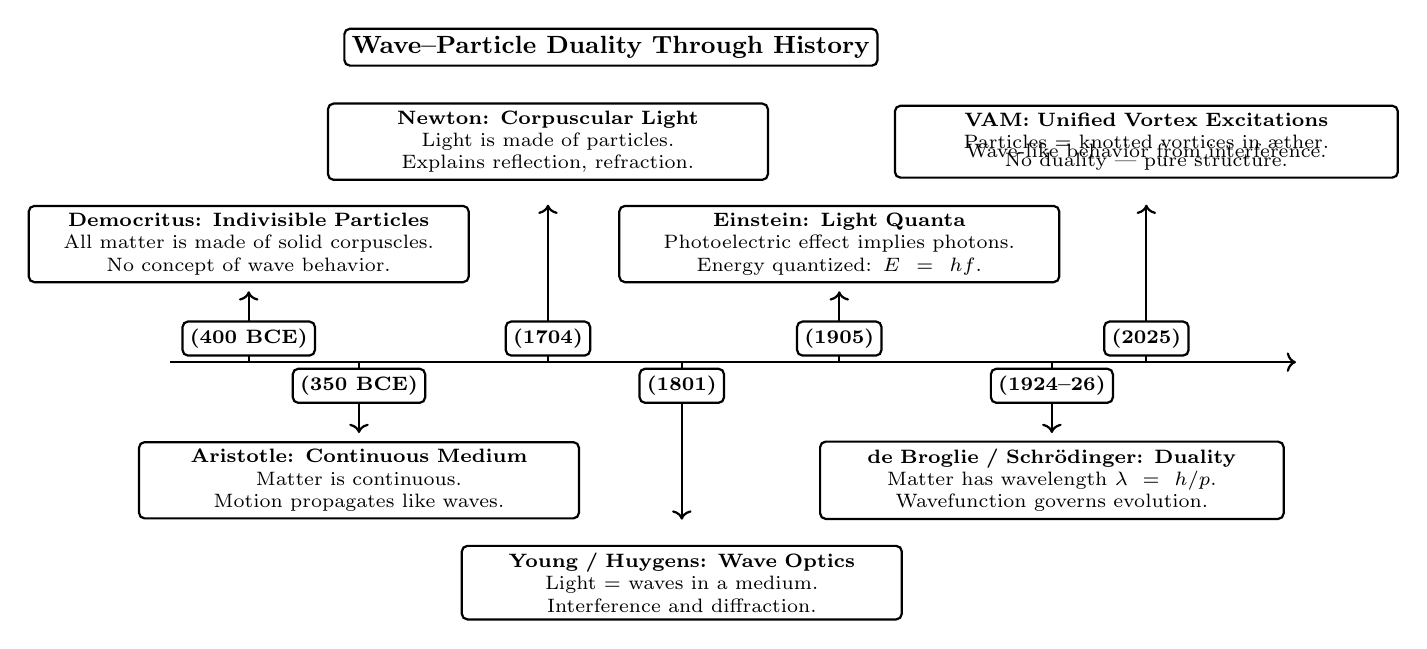
\begin{tikzpicture}
    \scriptsize

    % Timeline base
    \draw[->, thick] (-1,0) -- (13.3,0);

    % Arrows above timeline
    \draw[->, thick] (0,0) -- (0,0.9);       % Democritus
    \draw[->, thick] (3.8,0) -- (3.8,2.0);   % Newton
    \draw[->, thick] (7.5,0) -- (7.5,0.9);   % Einstein
    \draw[->, thick] (11.4,0) -- (11.4,2.0); % VAM

    % Arrows below timeline
    \draw[->, thick] (1.4,0) -- (1.4,-0.9);     % Aristotle
    \draw[->, thick] (5.5,0) -- (5.5,-2.0);     % Young/Huygens
    \draw[->, thick] (10.2,0) -- (10.2,-0.9);   % de Broglie

    % --- Date labels ---
    \node[draw, thick, rounded corners=2pt, fill=white, align=center, font=\bfseries ] at (0, .3)   {(400 BCE)};
    \node[draw, thick, rounded corners=2pt, fill=white, align=center, font=\bfseries ] at (3.8, .3) {(1704)};
    \node[draw, thick, rounded corners=2pt, fill=white, align=center, font=\bfseries ] at (7.5, .3) {(1905)};
    \node[draw, thick, rounded corners=2pt, fill=white, align=center, font=\bfseries ] at (11.4, .3){(2025)};

    \node[draw, thick, rounded corners=2pt, fill=white, align=center, font=\bfseries ] at (1.4,- .3) {(350 BCE)};
    \node[draw, thick, rounded corners=2pt, fill=white, align=center, font=\bfseries ] at (5.5,- .3) {(1801)};
    \node[draw, thick, rounded corners=2pt, fill=white, align=center, font=\bfseries ] at (10.2,- .3) {(1924--26)};

    % Timeline label
    \node[draw, thick, fill=white, rounded corners=2pt, font=\small] at (4.6,4.0) {\textbf{Wave–Particle Duality Through History}};

    % --- Democritus ---
    \node[draw, rounded corners=2pt, thick, align=center, fill=white, text width=5.4cm] at (0,1.5) {
    \textbf{Democritus: Indivisible Particles} \\% [-0.8em]
    All matter is made of solid corpuscles. \\% [-0.8em]
    No concept of wave behavior.
    };

    % --- Newton ---
    \node[draw, rounded corners=2pt, thick, align=center, fill=white, text width=5.4cm] at (3.8,2.8) {
    \textbf{Newton: Corpuscular Light} \\% [-0.8em]
    Light is made of particles. \\% [-0.8em]
    Explains reflection, refraction.
    };

    % --- Einstein ---
    \node[draw, rounded corners=2pt, thick, align=center, fill=white, text width=5.4cm] at (7.5,1.5) {
    \textbf{Einstein: Light Quanta} \\% [-0.8em]
    Photoelectric effect implies photons. \\% [-0.8em]
    Energy quantized: \( E = hf \).
    };

    % --- VAM ---
    \node[draw, rounded corners=2pt, thick, align=center, fill=white, text width=6.2cm] at (11.4,2.8) {
    \textbf{VAM: Unified Vortex Excitations} \\% [-0.8em]
    Particles = knotted vortices in æther. \\[-0.6em]
    Wave-like behavior from interference. \\[-0.6em]
    No duality — pure structure.
    };

    % --- Aristotle ---
    \node[draw, rounded corners=2pt, thick, align=center, fill=white, text width=5.4cm] at (1.4,-1.5) {
    \textbf{Aristotle: Continuous Medium} \\% [-0.8em]
    Matter is continuous. \\% [-0.8em]
    Motion propagates like waves.
    };

    % --- Young / Huygens ---
    \node[draw, rounded corners=2pt, thick, align=center, fill=white, text width=5.4cm] at (5.5,-2.8) {
    \textbf{Young / Huygens: Wave Optics} \\% [-0.8em]
    Light = waves in a medium. \\% [-0.8em]
    Interference and diffraction.
    };

    % --- de Broglie / Schrödinger ---
    \node[draw, rounded corners=2pt, thick, align=center, fill=white, text width=5.7cm] at (10.2,-1.5) {
    \textbf{de Broglie / Schrödinger: Duality} \\% [-0.8em]
    Matter has wavelength \( \lambda = h/p \). \\% [-0.8em]
    Wavefunction governs evolution.
    };

    \end{tikzpicture}
    \caption{\textbf{Intellectual trajectory of wave–particle duality:} from classical corpuscles and wave models to quantum dualities and beyond. VAM reframes the dichotomy by modeling all excitations as topologically structured vortices in a fluid æther. In this view, “particles” and “waves” are unified as geometric flow phenomena—dispensing with dualism in favor of pure structure.}\label{fig:WaveParticleDuality}
}


\subsection*[VAM-Derived Expression for G]{VAM-Derived Expression for G}

One of the notable results in VAM is a derivation of the gravitational constant in terms of ætheric and topological parameters~\cite{VAM-2, VAM-13, VAM-14}. Rewriting the expression in dimensionally transparent form:

\begin{equation}
    G_\text{swirl} = \frac{C_e}{2 F^{\max}_{\text{\ae}}} \cdot \left( \frac{c^5 t_p^2}{r_c^2} \right)
\end{equation}

\noindent where:
\begin{itemize}
    \item $C_e$: swirl velocity at the vortex boundary (m/s),
    \item $F^{\max}_{\text{\ae}}$: maximum force the æther can sustain before bifurcation (N),
    \item $t_p$: Planck time $ \left(\sqrt{\hbar G / c^5}\right) $,
    \item $r_c$: core radius of the vortex structure (m),
    \item $c$: speed of light in vacuum (m/s).
\end{itemize}

This formulation emerges from the Swirl Clock formalism and connects gravity to rotational energy density under conservation of circulation~
\cite{VAM-2, VAM-13}. It expresses $G$ not as a fundamental input constant, but as a derived quantity arising from the interplay of topological scale~\cite{bartini2005constants} $r_c$, rotational dynamics $C_e$, and ætheric tension $F^{\max}_{\text{\ae}}$. This reinforces the view that gravitation is a residual effect of conserved vorticity in a compressible ætheric medium. This formulation echoes recent emergent gravity approaches~\cite{Verlinde2011,Hossenfelder2017}, yet grounds gravity not in entropic gradients but in rotational conservation and swirl tension, which resonates with dynamical 3-space theories, in which gravity emerges from self-interacting spatial flow~\cite{cahill2003dynamical}.

VAM further incorporates circulation quantization, helicity conservation, and pressure-mediated interactions to model the exchange between knotted structures and their surrounding swirl fields~\cite{VAM-8, VAM-11, VAM-14}, consistent with nonlinear wave-vortex interaction theory in rotating fluids~\cite{buhler2005wave}. This general framework aligns with Einstein’s late attempt at a unified field theory—now realized through the mathematics of topological fluid dynamics.

The model's predictions are experimentally approachable through analog systems such as rotating superfluid vortices, BEC interference patterns, and refractive index shifts under swirl acceleration~\cite{VAM-2, VAM-13}. Such analogs mirror behavior seen in superfluid helium systems, including vortex quantization and phase discontinuities~\cite{tilley_superfluid}.  These offer testable pathways for validating the core dynamics proposed by VAM. These dynamics have observable analogs in superfluid and BEC systems, as described in analogue gravity programs~\cite{barcelo2005}.


\vspace{1em}

\section{Historical Continuity and Outlook}
A careful reexamination of Einstein's later writings reveals that he:
\begin{itemize}
    \item Did \emph{not} reject the æther outright, but \emph{redefined} it as a field-carrying substrate~\cite{einstein1920aether},
    \item Sought a \textbf{continuous medium} bearing the properties of spacetime without requiring mechanical motion,
    \item And ultimately pursued a \textbf{unified field theory}—one that VAM now echoes through the interplay of gravity, time perception, and vorticity~\cite{VAM-8, VAM-14}.
\end{itemize}

Einstein recognized that space could not be entirely void—it had to possess structural, energetic, and causal qualities. In this context, the Vortex Æther Model is not a speculative throwback, but a mathematically grounded continuation of Einstein's vision. It operationalizes this active structure via conserved vortex fields, topological knot invariants, and energy-sustaining boundary flows~\cite{VAM-8, VAM-11, VAM-14}.

While other contemporary models—such as emergent gravity and superfluid vacuum theory—have gestured toward similar foundations, VAM distinguishes itself by offering an explicitly solvable, hydrodynamically derived, and testable framework~\cite{VAM-8, VAM-14, VAM-15}. It bridges general relativity, thermodynamics, and quantum field heuristics without requiring discrete particles or quantized spacetime.

Kelvin's concern regarding topological degeneracy is addressed in Appendix~\ref{appendix:kelvin}.


\section*{Conclusion and Forward Outlook: Æther Reclaimed}

Modern theoretical physics is gradually converging on insights once considered obsolete—not because the underlying concepts were invalid, but because earlier mathematical and experimental tools lacked the necessary precision. Einstein’s late-career perspective on the æther anticipated this renaissance: a vision of space as a continuous, energetic, and causally structured medium. The Vortex Æther Model (VAM) builds directly on this foundation, advancing it into a unified, predictive, and testable framework~\cite{VAM-8, VAM-13, VAM-14}.

Here, vorticity and topological structure supplant the classical notion of curvature, and time itself emerges as a hierarchy of circulation and phase—fully realized in the multimodal temporal ontology~\cite{VAM-13, VAM-15}. The æther, once dismissed, returns in a new form: not as a mechanical ether, but as a quantized, causal, and observable substrate underlying all known phenomena—from gravitation and particle masses to quantum measurement and cosmological evolution~\cite{VAM-8, VAM-11, VAM-15}.

VAM does not merely offer a philosophical bridge to Einstein’s “unified field” dream, but delivers a rigorous technical foundation and explicit predictions that now invite empirical validation. With advancing experiments in superfluid analogues, quantum vortex interferometry, and photonic swirl, the opportunity to test, refine, or falsify these ideas moves within experimental reach~\cite{VAM-2, VAM-13, VAM-15}.

It is time to move beyond the view of Einstein as the man who abolished the æther, and instead to recognize him as the thinker who quietly reframed it—preparing the ground for its scientific rebirth. In that spirit, the Vortex Æther Model is not a closure, but an opening: a dynamic, empirically accessible, and mathematically coherent path forward in the ongoing quest for a unified physical theory.

\subsection*{Future Directions and Experimental Signatures}

The path forward for the Vortex Æther Model is both theoretically rich and experimentally accessible. On the theoretical front, continued development will further refine the topological classification of particle states~\cite{VAM-11, VAM-14}, explore fractal swirl dynamics at both quantum and cosmological scales~\cite{VAM-12, VAM-9}, and formalize the mechanisms by which gravitation and quantum phenomena emerge from circulation and helicity conservation~\cite{VAM-13, VAM-15}.

Empirically, the VAM framework provides several concrete predictions and signatures amenable to near-future tests:
\begin{itemize}
    \item \textbf{Time dilation and frame-dragging effects} in laboratory superfluids, Bose–Einstein condensates, and photonic vortex lattices~\cite{VAM-2, VAM-13};
    \item \textbf{Swirl clock phase slips and Kairos events} observable as quantized phase jumps or decoherence in quantum vortex interferometry~\cite{VAM-15};
    \item \textbf{Anomalous redshift, light bending, and perihelion precession} in astrophysical observations that deviate from standard General Relativity in high-vorticity or topologically complex environments~\cite{VAM-10};
    \item \textbf{Spectral and mass predictions} for leptons, baryons, and their excited states, determined by knot topology and quantized circulation~\cite{VAM-11, VAM-14};
    \item \textbf{Novel cosmological signatures} arising from large-scale swirl structure and the fractal dynamics of the æther, potentially visible in galaxy rotation curves and the cosmic microwave background~\cite{VAM-9, VAM-12}.
\end{itemize}

By combining theoretical coherence with falsifiable experimental predictions, the Vortex Æther Model opens a concrete research agenda for unifying gravitation, quantum mechanics, and cosmology. As the boundaries of precision measurement and analog simulation continue to expand, VAM stands poised to guide and interpret the next wave of discoveries at the intersection of topology, fluid dynamics, and fundamental physics.

\appendix

\section*{Appendix I: Helmholtz and the Foundations of Vortex Physics}
\label{appendix:helmholtz}
\addcontentsline{toc}{section}{Appendix I: Helmholtz on Vorticity}
    Hermann von Helmholtz’s 1858 paper \textit{“On the Integrals of the Hydrodynamic Equations Corresponding to Vortex Motion”}~\cite{helmholtz1858vortices} marks the formal beginning of vortex theory in physics. His theorems define the behavior of vorticity in an ideal, incompressible fluid—concepts foundational to the Vortex Æther Model (VAM).

    \subsection*{1. Vorticity is conserved along fluid lines}
    \begin{quote}
    \textit{“Each portion of a vortex filament remains connected to the same fluid elements throughout the motion.”}
    \end{quote}

    \textbf{VAM Mapping:} This becomes the core of VAM’s knot stability. Swirl identity is maintained via conserved helicity and circulation:
    \[
    \frac{d\Gamma}{dt} = 0, \quad \Gamma = \oint_{\mathcal{C}} \vec{v} \cdot d\vec{\ell}
    \]

    \subsection*{2. Vortex lines cannot end in a fluid — they form closed loops or extend to boundaries}
    \begin{quote}
    \textit{“The extremities of a vortex line cannot exist within the fluid; they must lie at the boundaries or form closed curves.”}
    \end{quote}

    \textbf{VAM Mapping:} Explains the closed-loop structure of particle-knot analogues in VAM. Vortices are topologically confined:
    \[
    \nabla \cdot \vec{\omega} = 0
    \]

    \subsection*{3. Circulation is invariant under ideal flow}
    \begin{quote}
    \textit{“The circulation around a closed curve moving with the fluid remains constant.”}
    \end{quote}

    \textbf{VAM Mapping:} VAM uses this to define internal clocks, mass, and swirl energy. This law becomes the origin of the time dilation formula:
    \[
    S(t) = \int \omega(t) \, dt, \quad T_v \sim \Gamma^{-1}
    \]

    \subsection*{Historical Legacy}

    Helmholtz's influence extended deeply into Kelvin’s vortex atom theory, Maxwell’s mechanical æther models, and later Einsteinian field theory. Today, in the Vortex Æther Model, his principles live on as conservation laws that define both structure and evolution of the physical vacuum.

    \begin{quote}
    \textit{“If matter is vortex, then Helmholtz is its first architect.”}
    \end{quote}
   \hfill — O. Iskandarani


\section*{Appendix II: Lord Kelvin and the Knot-Æther Critique}
\addcontentsline{toc}{section}{Appendix II: Lord Kelvin}
\label{appendix:kelvin}
   In the late 19th century, William Thomson (Lord Kelvin) proposed that atoms might be stable vortex knots in an invisible æther — a topological interpretation of matter. Yet he himself raised the most pointed critique:

   \begin{quote}
   `` I am afraid of the smoke and complication, of all the varieties of knots and links, if they are to explain the variety of elements.''
   \end{quote}
   \begin{flushright}
     — William Thomson (Lord Kelvin), Baltimore Lectures, 1890
   \end{flushright}

   Kelvin feared that the near-infinite number of possible knots and links in three-dimensional space would not correspond to the relatively small number of stable chemical elements~\cite{thomson1890knots, tait1877knots}. Without a natural principle of selection, the theory risked degeneracy: the proliferation of mathematically possible but physically irrelevant structures.

   \subsection*{Historical Context}

   In the second half of the 19th century, the vortex atom theory was developed, primarily by William Thomson (Lord Kelvin) and Peter Guthrie Tait~\cite{thomson1890knots, tait1877knots}. In this framework, atoms were envisioned as stable knots or vortex rings in an ideal, invisible fluid — the so-called luminiferous æther. The idea was that both the discrete nature of atomic species and their remarkable stability could be explained through topological invariants from knot theory.

   Helmholtz's 1858 paper introduced the conservation of vorticity in ideal fluids, laying the mathematical foundation upon which Kelvin and Tait constructed the vortex atom theory~\cite{helmholtz1858vortices}. This conservation principle is central to both classical vortex stability and the topological persistence employed in VAM.

   Kelvin's model was deeply influenced by the work of Helmholtz (1858) on vortex conservation in ideal fluids. He imagined that different types of knotted or linked vortices might correspond to different elements.

   \subsection*{Kelvin's Principal Objection}

   Despite its elegance, Kelvin identified a critical flaw:

   \begin{quote}
   `` I am afraid of the smoke and complication, of all the varieties of knots and links, if they are to explain the variety of elements.''
   \end{quote}
    \hfill — William Thomson (Lord Kelvin), Baltimore Lectures, 1890
   The mathematical space of knots is vast, and Kelvin recognized the absence of a physical filter. He was acutely aware that the theory, though geometrically rich, lacked a way to explain *why only some knots should be stable atoms*. It had no built-in energetic, dynamic, or entropic selection rule.

   \subsection*{Experimental Shortcomings}

   Kelvin also noted the absence of empirical correspondence between specific knot types and actual elements. Without experimental access to the supposed vortex knots — their formation, stability, or interaction — the theory remained speculative.

   Nonetheless, the idea lived on, inspiring both topological mathematics and future models of discrete matter arising from continuous media.

   \subsection*{Comparison to the Modern Particle Zoo}

   Kelvin's critique is echoed in modern particle physics. The Standard Model contains a large number of particles, generations, couplings, and constants — many set only by experimental input, not derivable from deeper principles.

   \begin{quote}
   \textit{`` I am afraid I must end by saying that the difficulties are so great in the way of forming anything like a comprehensive theory, that we cannot even imagine a finger-post pointing to a way that leads us towards the explanation.} \\
   \textit{But this time next year — this time ten years — this time one hundred years — I cannot doubt but that these things which now seem to us so mysterious will be no mysteries at all. The scales will fall from our eyes. We shall learn to look on things in a different way — when that which is now a difficulty will be the only common-sense and intelligible way of looking at the subject.''}
   \end{quote}
   \begin{flushright}
      — *Lord Kelvin, circa 1889*
   \end{flushright}


   The degeneracy Kelvin foresaw reappears: a theory with many admissible but unexplained types of particles. The need for a *selection mechanism* remains urgent.

   \subsection*{The VAM Response}

   The Vortex Æther Model (VAM) revives the topological atom intuition but answers Kelvin's critique with concrete physical principles:

   \begin{itemize}
     \item Thermodynamic constraints (via Clausius entropy) limit allowable knot growth~\cite{clausius1865entropy}.
     \item Quantized circulation excludes unstable, high-energy configurations.
     \item Absolute vorticity conservation enforces topological stability.
     \item Vortex reconnection thresholds act as evolutionary boundaries.
   \end{itemize}

   As a result, VAM predicts only a finite, physically meaningful spectrum of topological matter structures — in line with observed baryons and leptons.

   \subsection*{Concluding Reflection}

   Kelvin's objection was not to knots themselves, but to their uncontrolled proliferation. VAM reclaims his vision, but grounds it in hydrodynamic logic, energy bounds, and field evolution:

   \begin{quote}
    `` Knots without constraints become chaos. Knots with physics become atoms.''
   \end{quote}
      \begin{flushright}
      — O. Iskandarani
      \end{flushright}


\section*{Appendix III: James Clerk Maxwell on the Æther and the Vortex Atom Theory}
\addcontentsline{toc}{section}{Appendix III: James Clerk Maxwell on the Æther and the Vortex Atom Theory}
\label{appendix:maxwell}
 James Clerk Maxwell (1831–1879), one of the foundational figures of modern physics, held deep and evolving views on the concept of the æther. While best known for formulating the electromagnetic field equations, Maxwell also contributed to the theoretical underpinnings of the æther and engaged directly with the emerging vortex atom theories of his time.

 \subsection*{Maxwell's View on the Æther}
 Maxwell firmly believed that the æther was a physically real, omnipresent medium necessary for the transmission of electromagnetic waves~\cite{maxwell1878britannica}:

 \begin{quote}
 ``There can be no doubt that the interplanetary and interstellar spaces are not empty, but are occupied by a material substance\ldots which is certainly the largest and probably the most uniform body of which we have any knowledge.''
 \end{quote}

 To Maxwell, the electromagnetic field was not abstract, but a manifestation of real stresses and strains in the æther~\cite{maxwell1878britannica}. He imagined it as an elastic medium capable of supporting tension (electric fields), rotation (magnetic lines), and vibrational energy (light).

 \subsection*{Maxwell and the Vortex Atom Theory}

 Maxwell was intrigued by Lord Kelvin's proposal that atoms could be modeled as stable vortex knots in the æther — the so-called vortex atom theory~\cite{maxwell1875molecules}. In his 1875 lecture ``Molecules,'' he expressed qualified enthusiasm:

 \begin{quote}
 ``The vortex theory of atoms, first proposed by Helmholtz and developed by Sir William Thomson\ldots has made it conceivable that the properties of matter may depend solely on motion in a medium, and not on anything in the nature of the atom itself.''
 \end{quote}
\hfill — James Clerk Maxwell, 1875, ``Molecules''

 This radical idea — that all matter could emerge from organized motion in a universal fluid — deeply appealed to Maxwell's mechanical sensibilities. However, he also expressed caution:

 \begin{quote}
 ``The difficulty is that we know so little about fluid motion, and the equations are so intractable, that no one has yet been able to deduce the properties of any known substance from such a theory.''
 \end{quote}

 In short, the theory was conceptually beautiful but lacked mathematical tractability and predictive power. Maxwell understood the elegance of vortex-based models but noted that fluid dynamics was still too undeveloped to make the theory physically useful~\cite{maxwell1875molecules}.

 \subsection*{Legacy and Connection to VAM}

 Maxwell's æther was a mechanical medium filled with stresses, pressures, and circulations — not unlike the vortex fields described in the Vortex Æther Model (VAM). His aspirations for a unified field theory based on æther mechanics resonate strongly with VAM's goals:

 \begin{itemize}
   \item Both view the vacuum as structured and dynamic.
   \item Both describe matter as emergent from motion in the medium.
   \item Both seek to replace ad hoc constants with field-based origins.
 \end{itemize}

 Maxwell anticipated that future physicists might unlock the mathematics of vortex-structured æther. VAM — using conservation of vorticity, topological invariants, and pressure-induced time dilation — picks up where Maxwell's generation left off.

 \subsection*{Reflection}

 Maxwell's words remind us that the æther was never fully dismissed on scientific grounds, but rather due to limitations in modeling and experiment. With modern tools, those limitations are no longer insurmountable.

 \begin{quote}
 \textit{"A field is not a ghost. It is the visible strain of the invisible æther."}
 \end{quote}
 \hfill  — paraphrased from Maxwell's writings

\section*{Appendix IV: Einstein on the Æther — Translated Quotes and VAM Equivalents}
\addcontentsline{toc}{section}{Appendix IV: Einstein on the Æther}
\label{appendix:einstein}
This appendix collects and annotates key statements made by Albert Einstein about the æther, focusing especially on how these statements align or contrast with the structure and assumptions of the Vortex Æther Model (VAM). Where possible, original German excerpts are included, with English translations and a mapping to VAM concepts or equations.

\subsection*{1. ``Der Raum ohne Äther ist undenkbar..''}
\textbf{Original (1920 Leiden Lecture):} \\
``Nach der allgemeinen Relativitätstheorie ist der Raum mit physikalischen Eigenschaften begabt; in diesem Sinne existiert also ein Äther. Gemäß der allgemeinen Relativitätstheorie ist ein Raum ohne Äther undenkbar.''

\textbf{Translation:} \\
``According to the general theory of relativity, space is endowed with physical qualities; in this sense, therefore, there exists an æther. According to the general theory of relativity, space without æther is unthinkable.''

\textbf{VAM Mapping:} \\
This matches VAM's foundational postulate that the æther is a structured, non-viscous, incompressible medium with internal physical dynamics. The VAM equivalent is the existence of a vorticity-carrying background field \( \vec{\omega}(\vec{r}, t) \), subject to conservation laws and boundary conditions.

\[
\nabla \cdot \vec{v} = 0, \quad \nabla \cdot \vec{\omega} = 0, \quad \partial_t \vec{\omega} + (\vec{v} \cdot \nabla) \vec{\omega} = (\vec{\omega} \cdot \nabla) \vec{v}
\]

\subsection*{2. ``Es scheint, als sei die Einführung eines Äthers überflüssig...''}
\textbf{Original (1905, SR paper):} \\
``Es scheint, als sei die Einführung eines Äthers überflüssig, insofern die Lichtausbreitung durch Maxwell'sche Gleichungen in leerem Raum ausreichend beschrieben werden kann.''

\textbf{Translation:} \\
``It seems that the introduction of an æther is superfluous, insofar as the propagation of light can be described adequately by Maxwell's equations in vacuum.''

\textbf{VAM Mapping:} \\
Einstein's 1905 view was contextually specific to the Maxwellian field theory. VAM expands this to a \emph{sub-Maxwellian} fluid substrate: the fields emerge from vortex dynamics.

VAM introduces: \\
\( \vec{E} = -\nabla \Phi - \partial_t \vec{A}, \quad \vec{B} = \nabla \times \vec{A} \) as secondary fields derived from swirl-based potentials in the æther.

\subsection*{3. ``Der Äther darf nicht als ein Medium mit mechanischen Eigenschaften gedacht werden...''}
\textbf{Original (1920):} \\
``Der Äther darf nicht als ein Medium mit mechanischen Eigenschaften gedacht werden, wie es die alten Ätherkonzepte vorschlugen. Er besitzt keine Bewegungen, wie z.B. Geschwindigkeit.''

\textbf{Translation:} \\
``The æther must not be thought of as a medium with mechanical properties, as the old concepts of æther suggested. It has no motion in the usual sense, like velocity.''

\textbf{VAM Mapping:} \\
In VAM, the æther has \emph{field-like behavior}, not particulate or elastic-body behavior. The `` no absolute velocity'' principle is respected via invariance under global coordinate transformation, but local rotational states \( \vec{\omega} \neq 0 \) define structure. Time dilation depends on vorticity~\cite{VAM-2}:

\[
\frac{d\tau}{dt} = \sqrt{1 - \frac{C_e^2}{c^2} e^{-r/r_c}}
\]

\subsection*{4. ``Das Gravitationsfeld selbst kann als ein Zustand dieses Äthers angesehen werden.''}
\textbf{Original (1920):} \\
``Das Gravitationsfeld selbst kann als ein Zustand dieses Äthers angesehen werden.''

\textbf{Translation:} \\
``The gravitational field itself can be regarded as a state of this æther.''

\textbf{VAM Mapping:} \\
This is directly analogous to the VAM interpretation of gravity: not as spacetime curvature, but as an emergent effect of vorticity-induced pressure gradients:

\[
\nabla P = \rho_\text{\ae} \vec{a} = -\frac{1}{2} \rho_\text{\ae} \nabla |\vec{\omega}|^2
\]

\subsection*{5. ``Die Zeit ist in einem Gravitationsfeld anders definiert...''}
\textbf{Original (1916, Grundlagen der ART):} \\
``Die Zeit ist in einem Gravitationsfeld anders definiert als in der Abwesenheit desselben; die Zeitdifferenz hängt von der Lage im Feld ab.''

\textbf{Translation:} \\
``Time is defined differently in a gravitational field than in its absence; the time differential depends on the position within the field.''

\textbf{VAM Mapping:} \\
This statement supports VAM's approach of \emph{local time dilation} derived from rotational energy density and vorticity:

\[
\frac{d\tau}{dt} = \sqrt{1 - \frac{1}{U_\text{max}} U_{\text{vortex}}} = \sqrt{1 - \frac{1}{2U_\text{max}} \rho_\text{\ae} |\vec{\omega}|^2}
\]

\bigskip
\textit{ ``Einstein did not eliminate the æther. He redefined it. VAM takes the next step.''}\\
\hfill — O. Iskandarani\\

\section*{Appendix V: VAM Resolution of Einstein’s Final Æther Paradox}
\addcontentsline{toc}{section}{Appendix V: VAM and the Final Æther Paradox}
\label{appendix:final-aether}

\vspace{1em}

\begin{tcolorbox}[
    title={Einstein’s Final Æther Statement (1920)},
    colback=gray!7!white,
    colframe=black,
    boxrule=0.6pt,
    sharp corners=southwest,
    fonttitle=\bfseries,
    breakable
]
\begin{quote}
\small
“Space without æther is unthinkable; for in such space there not only would be no propagation of light, but also no possibility of existence for standards of space and time (measuring-rods and clocks), nor therefore any space-time intervals in the physical sense. But this æther may not be thought of as endowed with the quality characteristic of ponderable media, as consisting of parts which may be tracked through time. The idea of motion may not be applied to it.”
\end{quote}
\end{tcolorbox}

\vspace{0.6em}
\noindent
\textbf{The Paradox:} Einstein’s statement crystallizes his ultimate æther paradox: space must be endowed with physical qualities (an æther), yet the æther must possess \emph{no trackable motion}, no mechanical parts, and no temporally evolving components. The æther is thus essential but static—a silent scaffolding for relativistic structure.

\vspace{1em}

\begin{tcolorbox}[
    title={VAM Resolution: Internal Motion Without Bulk Translation},
    colback=gray!4!white,
    colframe=black,
    boxrule=0.6pt,
    sharp corners=southwest,
    fonttitle=\bfseries,
    breakable
]
The Vortex Æther Model (VAM) resolves this paradox by distinguishing between bulk translational motion and internal rotational structure:
\begin{itemize}
    \item The æther is \textbf{incompressible and inviscid}, preserving the continuum assumptions of fluid dynamics.
    \item It is \textbf{globally at rest} (\( \vec{v}_{\text{bulk}} = 0 \)), with no net velocity relative to absolute space.
    \item It is \textbf{locally dynamic}, supporting conserved vorticity and phase evolution:
    \[
        \boldsymbol{\omega} = \nabla \times \vec{v}, \qquad
        \vec{v}(r) = \frac{C_e}{r} e^{-r/r_c} \, \hat{\theta}
    \]
    \item It is \textbf{temporally causal}, with internal memory encoded in the swirl clock phase:
    \[
        \boldsymbol{S}(t) = \int \Omega(r) \, dt = \int \frac{C_e}{r_c} e^{-r/r_c} dt
    \]
\end{itemize}
No “parts” are tracked spatially, but topological invariants (vortex knots, helicity, linking number) serve as memory carriers—fulfilling Einstein’s requirements without violating his restrictions.
\end{tcolorbox}

\vspace{1em}

\begin{tcolorbox}[
    title={Clocks and Rods from Swirl Geometry},
    colback=gray!1!white,
    colframe=black,
    boxrule=0.6pt,
    sharp corners=southwest,
    fonttitle=\bfseries,
    breakable
]
Einstein argued that standards of space and time (measuring rods, clocks) require a nontrivial substrate. In VAM:
\begin{itemize}
    \item Both are emergent from local swirl structures. A “particle” is a \textbf{knotted vortex loop} with angular frequency \( \Omega \), circulation \( \Gamma \), and internal energy:
    \[
        U_{\text{vortex}} = \frac{1}{2} \rho_\text{\ae}^{(\text{energy})} |\boldsymbol{\omega}|^2
    \]
    \item Time dilation near such a structure follows:
    \[
        \frac{d\tau}{dt} = \sqrt{1 - \frac{U_{\text{vortex}}}{U_{\text{max}}}} = \sqrt{1 - \frac{1}{2U_{\text{max}}} \rho_\text{\ae}^{(\text{energy})} |\boldsymbol{\omega}|^2}
    \]
    \item Thus, “clocks” and “rods” are \emph{manifestations of local energetics and topology}, not primitive objects.
\end{itemize}
\end{tcolorbox}

\vspace{1em}

\begin{tcolorbox}[
    title={Reinterpreting “No Trackable Parts”},
    colback=gray!3!white,
    colframe=black,
    boxrule=0.6pt,
    sharp corners=southwest,
    fonttitle=\bfseries,
    breakable
]
Einstein forbade tracking “parts” of the æther through time. In VAM:
\begin{itemize}
    \item Fluid elements are not tracked by position;
    \item Instead, \textbf{vortex filaments} and their topological invariants (\( \ell \), \( H \), \( K \)) encode causal evolution and system memory;
    \item These are not particulate—they are \emph{topological excitations}, reconciling Einstein’s view with a physically rich substrate.
\end{itemize}
\end{tcolorbox}

\vspace{1em}

\begin{tcolorbox}[
    title={Conclusion: From Silent Substrate to Structured Swirl},
    colback=gray!8!white,
    colframe=black,
    boxrule=0.6pt,
    sharp corners=southwest,
    fonttitle=\bfseries,
    breakable
]
Where Einstein’s æther was a silent backdrop enabling relativity, VAM’s æther is an \emph{active but non-translating medium} whose internal structure encodes mass, time, inertia, and gravity.
\vspace{0.5em}

\textit{“Einstein stripped the æther of velocity to preserve symmetry. VAM restores internal motion to recover substance.”}
\begin{flushright}
— O. Iskandarani
\end{flushright}
\end{tcolorbox}

\section{Simultaneity: From Light Pulses to Vortex Clocks}
    In Einstein’s theory, time is defined operationally through the arrival and departure of light signals. Simultaneity is not absolute, but constructed by coordinating photon trajectories between clocks. This makes time a relational concept—dependent on the motion of observers and the invariance of light speed.

    \begin{table}[h!]
        \centering
        \begin{tabular}{|c|c|c|c|}
            \hline
            \textbf{Theory} & \textbf{Time} & \textbf{Simultaneity} & \textbf{Defined By} \\
            \hline
            Newton & Absolute & Universal & External flow of time \\
            Einstein (SR/GR) & Relative & Frame-dependent & Light signal coordination \\
            VAM & Layered (N, $\tau$, $S(t)$) & Phase-coherent & Vortex swirl phase $\Omega(r)$ \\
            \hline
        \end{tabular}
        \caption{Comparison of time and simultaneity in Newtonian, Einsteinian, and VAM frameworks.}
    \end{table}

    In contrast, the Vortex Æther Model grounds time in the internal dynamics of the medium itself. Absolute æther time \( N \) flows uniformly, while local time \( \tau \) and swirl clock time \( S(t) \) emerge from the rotational energy and helicity of vortex structures. Simultaneity is no longer a matter of synchronization via photons—it is encoded in the shared phase coherence of knotted circulation. In this sense, VAM replaces relativistic light-clock simultaneity with a topologically grounded, energetically conserved temporal ontology.



\begin{figure}[htbp]
      \centering
    \scriptsize
        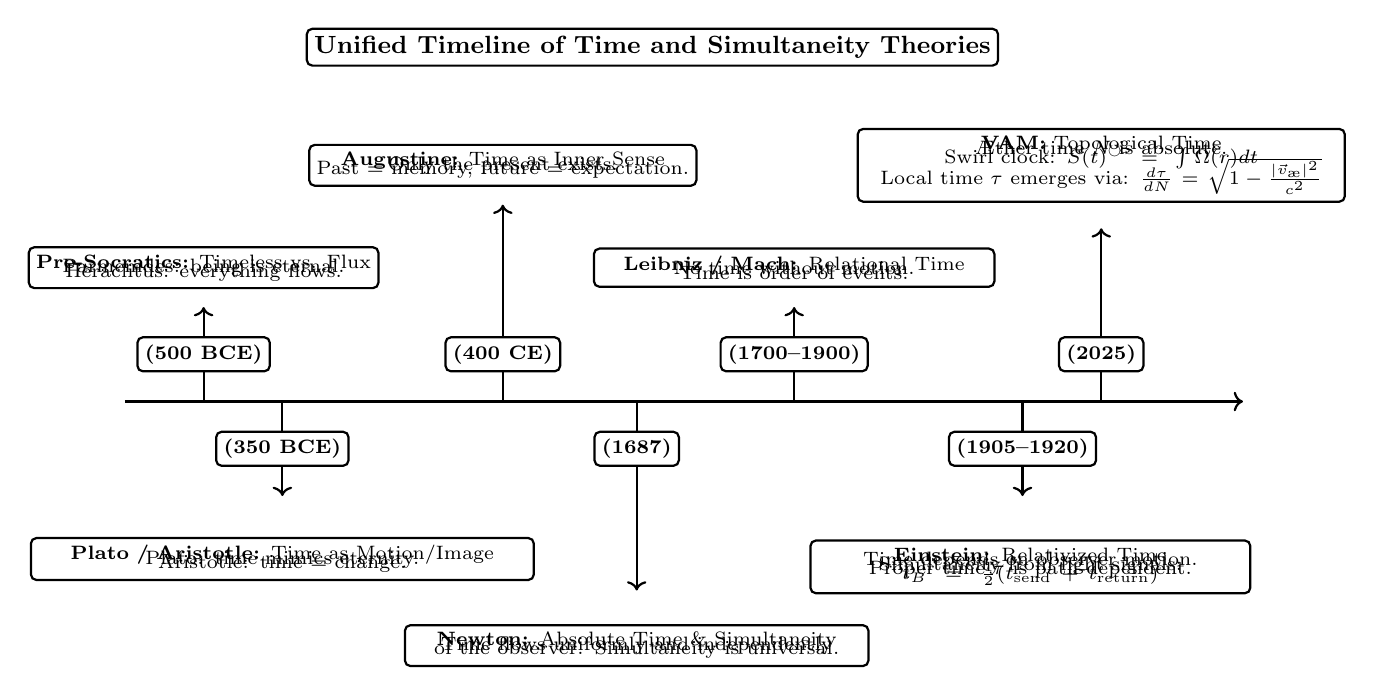
\begin{tikzpicture}
        \scriptsize
        % Timeline base
        \draw[->, thick] (-1,0) -- (13.2,0);

        % Arrows above timeline (short, as requested)
        \draw[->, thick] (0,0) -- (0,1.2);       % Pre-Socratics
        \draw[->, thick] (3.8,0) -- (3.8,2.5);   % Augustine
        \draw[->, thick] (7.5,0) -- (7.5,1.2);   % Einstein
        \draw[->, thick] (11.4,0) -- (11.4,2.2); % VAM

        % Arrows below timeline (short, as requested)
        \draw[->, thick] (1.0,0) -- (1.0,-1.2);     % Plato/Aristotle
        \draw[->, thick] (5.5,0) -- (5.5,-2.4);     % Newton
        \draw[->, thick] (10.4,0) -- (10.4,-1.2);     % Leibniz/Mach

            %--- Root title cards (above timeline) ---
        \node[draw, thick, rounded corners=2pt, fill=white, align=center, font=\bfseries ] at (0, .6)   {(500 BCE)};
        \node[draw, thick, rounded corners=2pt, fill=white, align=center, font=\bfseries ] at (3.8, .6) {(400 CE)};
        \node[draw, thick, rounded corners=2pt, fill=white, align=center, font=\bfseries ] at (7.5, .6) {(1700--1900)};
        \node[draw, thick, rounded corners=2pt, fill=white, align=center, font=\bfseries ] at (11.4, .6){(2025)};

        %--- Root title cards (below timeline) ---
        \node[draw, thick, rounded corners=2pt, fill=white, align=center, font=\bfseries ] at (1.0,- .6) {(350 BCE)};
        \node[draw, thick, rounded corners=2pt, fill=white, align=center, font=\bfseries ] at (5.5,- .6) {(1687)};
        \node[draw, thick, rounded corners=2pt, fill=white, align=center, font=\bfseries ] at (10.4,- .6) {(1905--1920)};

            % Timeline label
        \node[draw, thick, fill=white, rounded corners=2pt, font=\small] at (5.7,4.5) {\textbf{Unified Timeline of Time and Simultaneity Theories}};

        % --- Pre-Socratics ---
        \node[draw, rounded corners=2pt, thick, align=center, fill=white] at (0,1.7) {
        \textbf{Pre-Socratics:} Timeless vs. Flux \\[-0.8em]
        Parmenides: being is eternal. \\[-0.8em]
        Heraclitus: everything flows.
        };

        % --- Augustine ---
        \node[draw, rounded corners=2pt, thick, align=center, fill=white] at (3.8,3.0) {
        \textbf{Augustine:} Time as Inner Sense \\[-0.8em]
        Only the present exists. \\[-0.8em]
        Past = memory, future = expectation.
        };

        % --- Leibniz / Mach ---
        \node[draw, rounded corners=2pt, thick, align=center, fill=white, text width=4.9cm] at (7.5,1.7) {
        \textbf{Leibniz / Mach:} Relational Time \\[-0.8em]
        No time without motion. \\[-0.8em]
        Time is order of events.
        };
        % --- VAM (modern) ---
        \node[draw, rounded corners=2pt, thick, align=center, fill=white, text width=6.0cm] at (11.4,3.0) {
        \textbf{VAM:} Topological Time \\[-0.8em]
        Æther time $N$ is absolute. \\[-0.6em]
        Swirl clock: $S(t)^\circlearrowleft = \int \Omega(r) dt$ \\[-0.6em]
        Local time $\tau$ emerges via: $ \frac{d\tau}{dN} = \sqrt{1 - \frac{|\vec{v}_\text{\ae}|^2}{c^2}}$

        };


        % --- Plato / Aristotle ---
        \node[draw, rounded corners=2pt, thick, align=center, fill=white, text width=6.2cm] at (1.0,-2) {
        \textbf{Plato / Aristotle:} Time as Motion/Image \\[-0.8em]
        Plato: time mimics eternity. \\[-0.8em]
        Aristotle: time = change.
        };



        % --- Einstein ---
        \node[draw, rounded corners=2pt, thick, align=center, fill=white, text width=5.4cm] at (10.5,-2.1) {
        \textbf{Einstein:} Relativized Time \\[-0.8em]
        Time depends on observer motion. \\[-0.8em]
        Simultaneity from light signals: \\[-0.8em]
        Proper time $\tau$ is path-dependent.\\[-0.8em]
        $t_B = \frac{1}{2}(t_{\text{send}} + t_{\text{return}})$
        };

        % --- Newton ---
        \node[draw, rounded corners=2pt, thick, align=center, fill=white, text width=5.7cm] at (5.5,-3.1) {
        \textbf{Newton:} Absolute Time \& Simultaneity \\[-0.8em]
        Time flows uniformly and independently \\[-0.8em]
        of the observer. Simultaneity is universal.
        };
         \end{tikzpicture}
        \caption{Fused history of time and simultaneity: from early philosophical views and Newton’s absolutes to Einstein’s relativistic structure and VAM’s layered, swirl-based temporality.}\label{fig:history-time-simultaneity}
\end{figure}

\resizebox{\textwidth}{!}{%
      \centering
    \scriptsize
    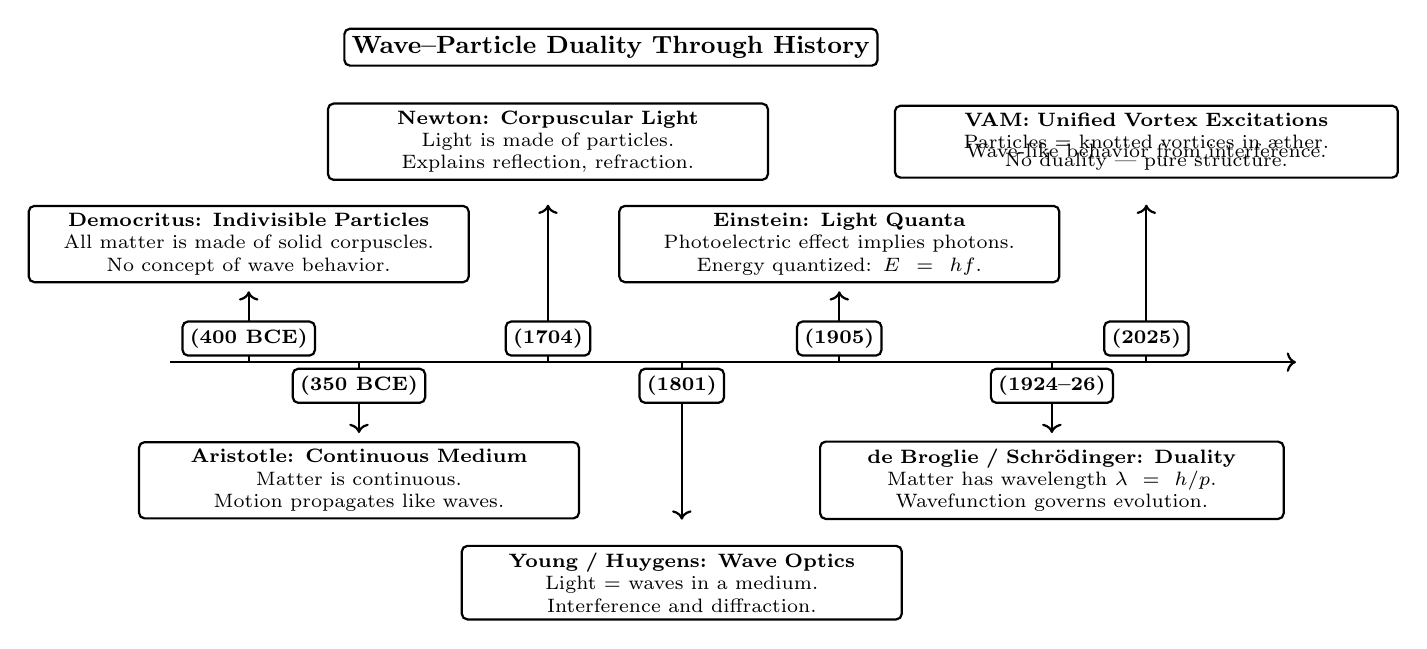
\begin{tikzpicture}
    \scriptsize

    % Timeline base
    \draw[->, thick] (-1,0) -- (13.3,0);

    % Arrows above timeline
    \draw[->, thick] (0,0) -- (0,0.9);       % Democritus
    \draw[->, thick] (3.8,0) -- (3.8,2.0);   % Newton
    \draw[->, thick] (7.5,0) -- (7.5,0.9);   % Einstein
    \draw[->, thick] (11.4,0) -- (11.4,2.0); % VAM

    % Arrows below timeline
    \draw[->, thick] (1.4,0) -- (1.4,-0.9);     % Aristotle
    \draw[->, thick] (5.5,0) -- (5.5,-2.0);     % Young/Huygens
    \draw[->, thick] (10.2,0) -- (10.2,-0.9);   % de Broglie

    % --- Date labels ---
    \node[draw, thick, rounded corners=2pt, fill=white, align=center, font=\bfseries ] at (0, .3)   {(400 BCE)};
    \node[draw, thick, rounded corners=2pt, fill=white, align=center, font=\bfseries ] at (3.8, .3) {(1704)};
    \node[draw, thick, rounded corners=2pt, fill=white, align=center, font=\bfseries ] at (7.5, .3) {(1905)};
    \node[draw, thick, rounded corners=2pt, fill=white, align=center, font=\bfseries ] at (11.4, .3){(2025)};

    \node[draw, thick, rounded corners=2pt, fill=white, align=center, font=\bfseries ] at (1.4,- .3) {(350 BCE)};
    \node[draw, thick, rounded corners=2pt, fill=white, align=center, font=\bfseries ] at (5.5,- .3) {(1801)};
    \node[draw, thick, rounded corners=2pt, fill=white, align=center, font=\bfseries ] at (10.2,- .3) {(1924--26)};

    % Timeline label
    \node[draw, thick, fill=white, rounded corners=2pt, font=\small] at (4.6,4.0) {\textbf{Wave–Particle Duality Through History}};

    % --- Democritus ---
    \node[draw, rounded corners=2pt, thick, align=center, fill=white, text width=5.4cm] at (0,1.5) {
    \textbf{Democritus: Indivisible Particles} \\% [-0.8em]
    All matter is made of solid corpuscles. \\% [-0.8em]
    No concept of wave behavior.
    };

    % --- Newton ---
    \node[draw, rounded corners=2pt, thick, align=center, fill=white, text width=5.4cm] at (3.8,2.8) {
    \textbf{Newton: Corpuscular Light} \\% [-0.8em]
    Light is made of particles. \\% [-0.8em]
    Explains reflection, refraction.
    };

    % --- Einstein ---
    \node[draw, rounded corners=2pt, thick, align=center, fill=white, text width=5.4cm] at (7.5,1.5) {
    \textbf{Einstein: Light Quanta} \\% [-0.8em]
    Photoelectric effect implies photons. \\% [-0.8em]
    Energy quantized: \( E = hf \).
    };

    % --- VAM ---
    \node[draw, rounded corners=2pt, thick, align=center, fill=white, text width=6.2cm] at (11.4,2.8) {
    \textbf{VAM: Unified Vortex Excitations} \\% [-0.8em]
    Particles = knotted vortices in æther. \\[-0.6em]
    Wave-like behavior from interference. \\[-0.6em]
    No duality — pure structure.
    };

    % --- Aristotle ---
    \node[draw, rounded corners=2pt, thick, align=center, fill=white, text width=5.4cm] at (1.4,-1.5) {
    \textbf{Aristotle: Continuous Medium} \\% [-0.8em]
    Matter is continuous. \\% [-0.8em]
    Motion propagates like waves.
    };

    % --- Young / Huygens ---
    \node[draw, rounded corners=2pt, thick, align=center, fill=white, text width=5.4cm] at (5.5,-2.8) {
    \textbf{Young / Huygens: Wave Optics} \\% [-0.8em]
    Light = waves in a medium. \\% [-0.8em]
    Interference and diffraction.
    };

    % --- de Broglie / Schrödinger ---
    \node[draw, rounded corners=2pt, thick, align=center, fill=white, text width=5.7cm] at (10.2,-1.5) {
    \textbf{de Broglie / Schrödinger: Duality} \\% [-0.8em]
    Matter has wavelength \( \lambda = h/p \). \\% [-0.8em]
    Wavefunction governs evolution.
    };

    \end{tikzpicture}
    \caption{\textbf{Intellectual trajectory of wave–particle duality:} from classical corpuscles and wave models to quantum dualities and beyond. VAM reframes the dichotomy by modeling all excitations as topologically structured vortices in a fluid æther. In this view, “particles” and “waves” are unified as geometric flow phenomena—dispensing with dualism in favor of pure structure.}\label{fig:WaveParticleDuality}
}
\begin{center}
\footnotesize
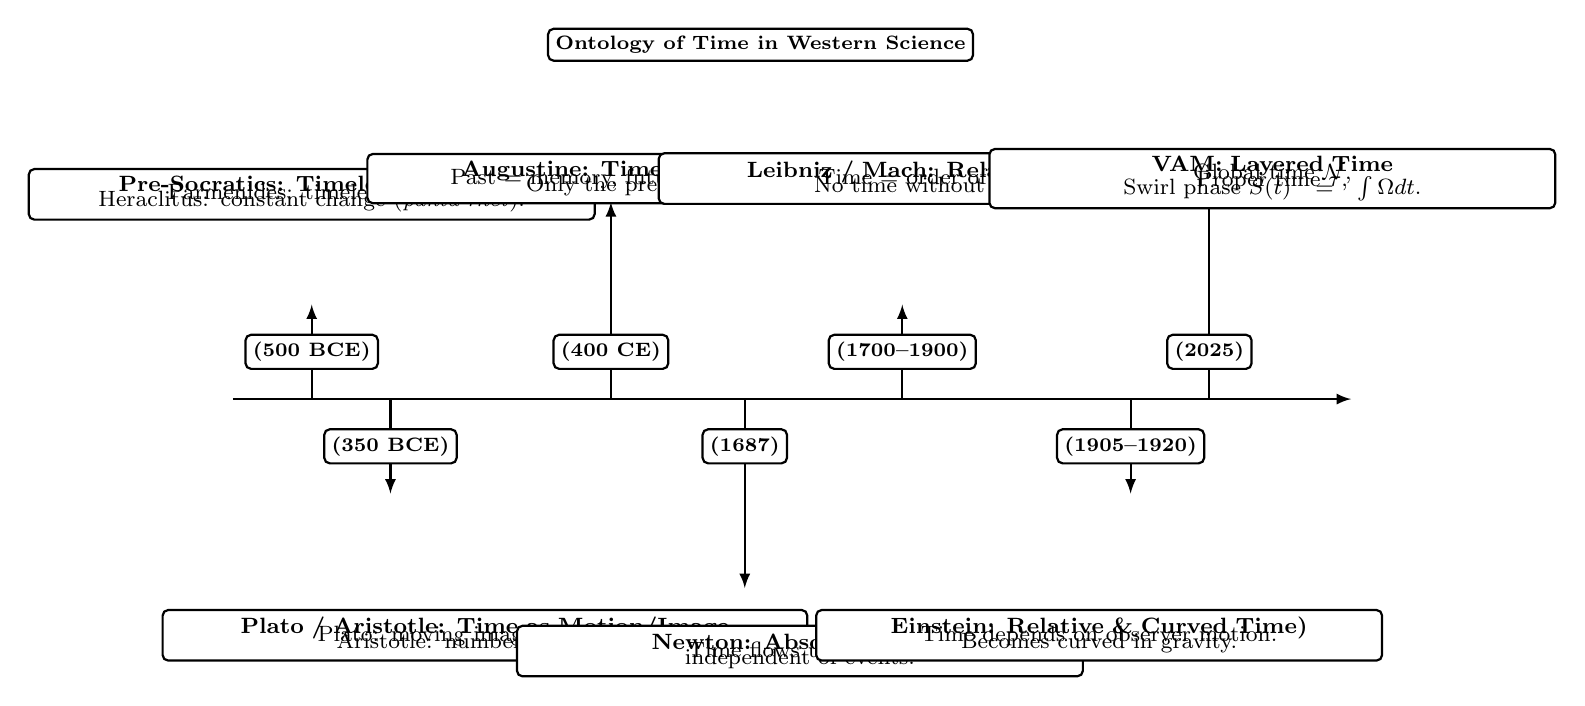
\begin{tikzpicture}[node distance=3.5cm, every node/.style={font=\footnotesize}, >=latex]
\scriptsize


% Timeline base
\draw[->, thick] (-1,0) -- (13.2,0);

% Arrows above timeline (short, as requested)
\draw[->, thick] (0,0) -- (0,1.2);       % Pre-Socratics
\draw[->, thick] (3.8,0) -- (3.8,2.5);   % Augustine
\draw[->, thick] (7.5,0) -- (7.5,1.2);   % Einstein
\draw[->, thick] (11.4,0) -- (11.4,3.0); % VAM

% Arrows below timeline (short, as requested)
\draw[->, thick] (1.0,0) -- (1.0,-1.2);     % Plato/Aristotle
\draw[->, thick] (5.5,0) -- (5.5,-2.4);     % Newton
\draw[->, thick] (10.4,0) -- (10.4,-1.2);     % Leibniz/Mach

    %--- Root title cards (above timeline) ---
\node[draw, thick, rounded corners=2pt, fill=white, align=center, font=\bfseries ] at (0, .6)   {(500 BCE)};
\node[draw, thick, rounded corners=2pt, fill=white, align=center, font=\bfseries ] at (3.8, .6) {(400 CE)};
\node[draw, thick, rounded corners=2pt, fill=white, align=center, font=\bfseries ] at (7.5, .6) {(1700--1900)};
\node[draw, thick, rounded corners=2pt, fill=white, align=center, font=\bfseries ] at (11.4, .6){(2025)};

%--- Root title cards (below timeline) ---
\node[draw, thick, rounded corners=2pt, fill=white, align=center, font=\bfseries ] at (1.0,- .6) {(350 BCE)};
\node[draw, thick, rounded corners=2pt, fill=white, align=center, font=\bfseries ] at (5.5,- .6) {(1687)};
\node[draw, thick, rounded corners=2pt, fill=white, align=center, font=\bfseries ] at (10.4,- .6) {(1905--1920)};

% Label (centered box)
\node[draw, thick, fill=white, rounded corners=2pt, font=\scriptsize] at (5.7,4.5) {\textbf{Ontology of Time in Western Science}};

% Ancient Greek: Parmenides / Heraclitus
\node[draw, rounded corners=2pt, thick, align=center, fill=white, text width=7cm] at (0,2.6) {
\textbf{Pre-Socratics: Timeless vs. Flux}  \\[-0.8em]
Parmenides: timeless being.  \\[-0.8em]
Heraclitus: constant change (\textit{panta rhei}).
};

% Plato / Aristotle
\node[draw, rounded corners=2pt, thick, align=center, fill=white, text width=8cm] at (2.2,-3.0) {
\textbf{Plato / Aristotle: Time as Motion/Image}  \\[-0.8em]
Plato: moving image of eternity.  \\[-0.8em]
Aristotle: number of change.
};

% Augustine
\node[draw, rounded corners=2pt, thick, align=center, fill=white, text width=7cm] at (4.3,2.8) {
\textbf{Augustine: Time as Inner Sense}  \\[-0.8em]
Past = memory, future = anticipation.  \\[-0.8em]
Only the present is real.
};

% Newton
\node[draw, rounded corners=2pt, thick, align=center, fill=white, text width=7cm] at (6.2,-3.2) {
\textbf{Newton: Absolute Time)}  \\[-0.8em]
Time flows uniformly,  \\[-0.8em]
independent of events.
};


% Relationalists: Leibniz / Mach
\node[draw, rounded corners=2pt, thick, align=center, fill=white, text width=7cm] at (8.0,2.8) {
\textbf{Leibniz / Mach: Relational Time}  \\[-0.8em]
Time = order of events.  \\[-0.8em]
No time without change.
};

% Einstein
\node[draw, rounded corners=2pt, thick, align=center, fill=white, text width=7cm] at (10.0,-3.0) {
\textbf{Einstein: Relative \& Curved Time)}  \\[-0.8em]
Time depends on observer motion.  \\[-0.8em]
Becomes curved in gravity.
};


% VAM
\node[draw, rounded corners=2pt, thick, align=center, fill=white, text width=7cm] at (12.2,2.8) {
\textbf{VAM: Layered Time}  \\[-0.8em]
Global time \( \mathcal{N} \),  \\[-0.8em]
Proper time \( \tau \),  \\[-0.8em]
Swirl phase \( S(t) = \int \Omega dt \).
};


\end{tikzpicture}
\captionof{figure}{Historical evolution of temporal ontology: from pre-Socratic polarity to Einstein's spacetime and the layered temporality of the Vortex Æther Model.}
\end{center}
\begin{figure}[htbp]
      \centering
    \scriptsize
    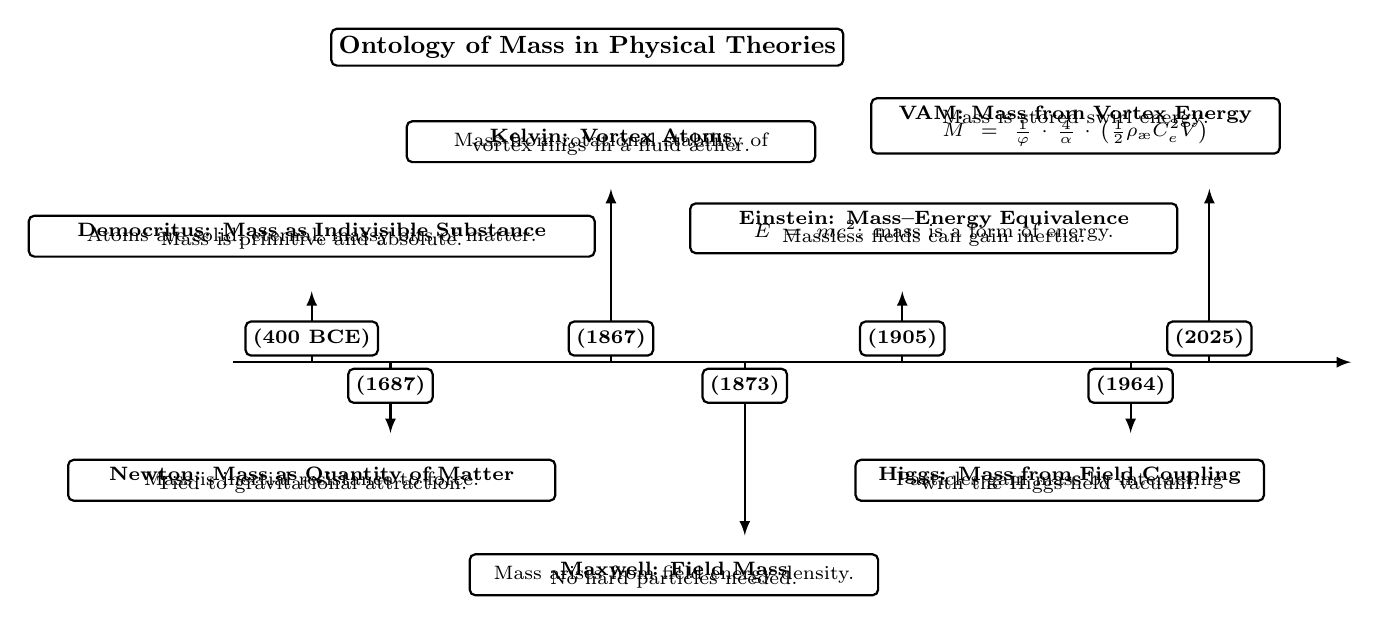
\begin{tikzpicture}[node distance=3.5cm, every node/.style={font=\scriptsize}, >=latex]
    \scriptsize

    % Timeline base
    \draw[->, thick] (-1,0) -- (13.2,0);

    % Arrows above timeline (short, as requested)
    \draw[->, thick] (0,0) -- (0,0.9);       % Pre-Socratics
    \draw[->, thick] (3.8,0) -- (3.8,2.2);   % Augustine
    \draw[->, thick] (7.5,0) -- (7.5,0.9);   % Einstein
    \draw[->, thick] (11.4,0) -- (11.4,2.2); % VAM

    % Arrows below timeline (short, as requested)
    \draw[->, thick] (1.0,0) -- (1.0,-0.9);     % Plato/Aristotle
    \draw[->, thick] (5.5,0) -- (5.5,-2.2);     % Newton
    \draw[->, thick] (10.4,0) -- (10.4,-0.9);     % Leibniz/Mach

        %--- Root title cards (above timeline) ---
    \node[draw, thick, rounded corners=2pt, fill=white, align=center, font=\bfseries ] at (0, .3)   {(400 BCE)};
    \node[draw, thick, rounded corners=2pt, fill=white, align=center, font=\bfseries ] at (3.8, .3) {(1867)};
    \node[draw, thick, rounded corners=2pt, fill=white, align=center, font=\bfseries ] at (7.5, .3) {(1905)};
    \node[draw, thick, rounded corners=2pt, fill=white, align=center, font=\bfseries ] at (11.4, .3){(2025)};

    %--- Root title cards (below timeline) ---
    \node[draw, thick, rounded corners=2pt, fill=white, align=center, font=\bfseries ] at (1.0,- .3) {(1687)};
    \node[draw, thick, rounded corners=2pt, fill=white, align=center, font=\bfseries ] at (5.5,- .3) {(1873)};
    \node[draw, thick, rounded corners=2pt, fill=white, align=center, font=\bfseries ] at (10.4,- .3) {(1964)};

    % Label
    \node[draw, thick, fill=white, rounded corners=2pt, font=\small] at (3.5,4.0) {\textbf{Ontology of Mass in Physical Theories}};

    % Democritus (left)
    \node[draw, rounded corners=2pt, thick, align=center, fill=white, text width=7cm] at (0,1.6) {
    \textbf{Democritus: Mass as Indivisible Substance}  \\[-0.8em]
    Atoms are solid, eternal, massy bits of matter.  \\[-0.8em]
    Mass is primitive and absolute.
    };

    % Newton (below)
    \node[draw, rounded corners=2pt, thick, align=center, fill=white, text width=6cm] at (0,-1.5) {
    \textbf{Newton: Mass as Quantity of Matter}  \\[-0.8em]
    Mass is inertial resistance to force.  \\[-0.8em]
    Tied to gravitational attraction.
    };


    % Kelvin (top)
    \node[draw, rounded corners=2pt, thick, align=center, fill=white, text width=5cm] at (3.8,2.8) {
    \textbf{Kelvin: Vortex Atoms}  \\[-0.8em]
    Mass from rotational stability of  \\[-0.8em]
    vortex rings in a fluid æther.
    };


    % Maxwell (bottom)
    \node[draw, rounded corners=2pt, thick, align=center, fill=white, text width=5cm] at (4.6,-2.7) {
    \textbf{Maxwell: Field Mass}  \\[-0.8em]
    Mass arises from field energy density.  \\[-0.8em]
    No hard particles needed.
    };

    % Einstein (top)
    \node[draw, rounded corners=2pt, thick, align=center, fill=white, text width=6cm] at (7.9,1.7) {
    \textbf{Einstein: Mass–Energy Equivalence}  \\[-0.4em]
    \( E = mc^2 \): mass is a form of energy.  \\[-0.8em]
    Massless fields can gain inertia.
    };


    % Higgs (bottom)
    \node[draw, rounded corners=2pt, thick, align=center, fill=white, text width=5cm] at (9.5,-1.5) {
    \textbf{Higgs: Mass from Field Coupling}  \\[-0.8em]
    Particles gain mass by interacting  \\[-0.8em]
    with the Higgs field vacuum.
    };


    % VAM (top right)
    \node[draw, rounded corners=2pt, thick, align=center, fill=white, text width=5cm] at (9.7,3.0) {
    \textbf{VAM: Mass from Vortex Energy}  \\[-0.8em]
    Mass is stored swirl energy:  \\[-0.4em]
    \( M = \frac{1}{\varphi} \cdot \frac{4}{\alpha} \cdot \left( \frac{1}{2} \rho_\text{\ae} C_e^2 V \right) \)
    };

    \end{tikzpicture}
    \caption{\textbf{Evolution of the concept of mass across physics:} from atomistic substance (Democritus), through Newtonian inertia and field-theoretic mass (Maxwell, Higgs), to VAM’s fluid-topological model. In VAM, mass is emergent swirl energy stored in knotted vortex configurations within a quantized æther. Each stage reflects deeper abstraction—from particles to energy to geometry to topology.}\label{fig:OntologyOfMass}
\end{figure}

\section*{Final Reflection: Æther Past and Future}

    These appendices trace a conceptual lineage—beginning with Maxwell's mechanical æther as a carrier of field stresses, evolving through Kelvin's vision of atoms as knotted vortex rings, and reformulated by Einstein into a geometric substrate underlying spacetime itself. Each step preserved the core intuition: that empty space is not truly empty, but possesses structure, energy, and dynamical influence.

    The Vortex Æther Model (VAM) completes this lineage by merging the fluid and field paradigms into a unified topological framework. In VAM, the æther is no longer an abstract scaffolding or discarded relic, but a physically real medium: incompressible, inviscid, and threaded with quantized vorticity. Mass arises from rotational energy; gravity from swirl-induced pressure gradients; time from the internal phase of topological knots.

    Where previous æther models lacked formal consistency or empirical validation, VAM draws on modern tools—fluid dynamics, knot theory, Hamiltonian flows, and high-precision measurement—to revisit the æther hypothesis with scientific rigor and predictive power.

    Einstein redefined the æther without abandoning it. VAM takes the next step—restoring motion, structure, and causality to the medium beneath all physical law.



    \bibliographystyle{unsrt}
    \bibliography{VAM-0-From_Einstein_to_the_Vortex_Fluid_paradigm}
\end{document}